\documentclass[12pt]{article}

% ---- preámbulo básico compatible con pdflatex ----
\usepackage[spanish]{babel}
\usepackage[utf8]{inputenc}
\usepackage[T1]{fontenc}
\usepackage[a4paper,margin=1in]{geometry}
\usepackage{graphicx}
\usepackage{float}
\usepackage[hidelinks]{hyperref}

% compilar con working dir = C:/textdata/post
\graphicspath{{./figuras/}}

\title{UMass Amherst -- Tesis (2009--presente)\\
	\large Advisors y foco temático en el trabajo de James K.~Boyce}
\author{Diego Polanco}
\date{\today}

\begin{document}
	\maketitle
	
	\section{Construí una base de las tesis usando webscrapping}
	Reuní una base con metadatos de tesis doctorales del Departamento de Economía de UMass Amherst. El objetivo fue capturar título, año, hasta cinco posiciones de \textit{advisor} y el \textit{abstract}. Los nombres de advisors fueron estandarizados y se limpiaron valores basura.
	
	\section{La base incluye abstracts y advisors desde 2009}
	El repositorio es consistente a partir de 2009. Todo el análisis se restringe a ese período para evitar sesgos de cobertura.
	
	\section{James K.~Boyce aparece como el economista más influyente (main advisor)}
	La figura resume el ranking de \textit{main advisors} desde 2009. En términos de dirección principal de tesis, James K.~Boyce lidera con holgura respecto del resto del cuerpo académico.
	
	\begin{figure}[H]\centering
		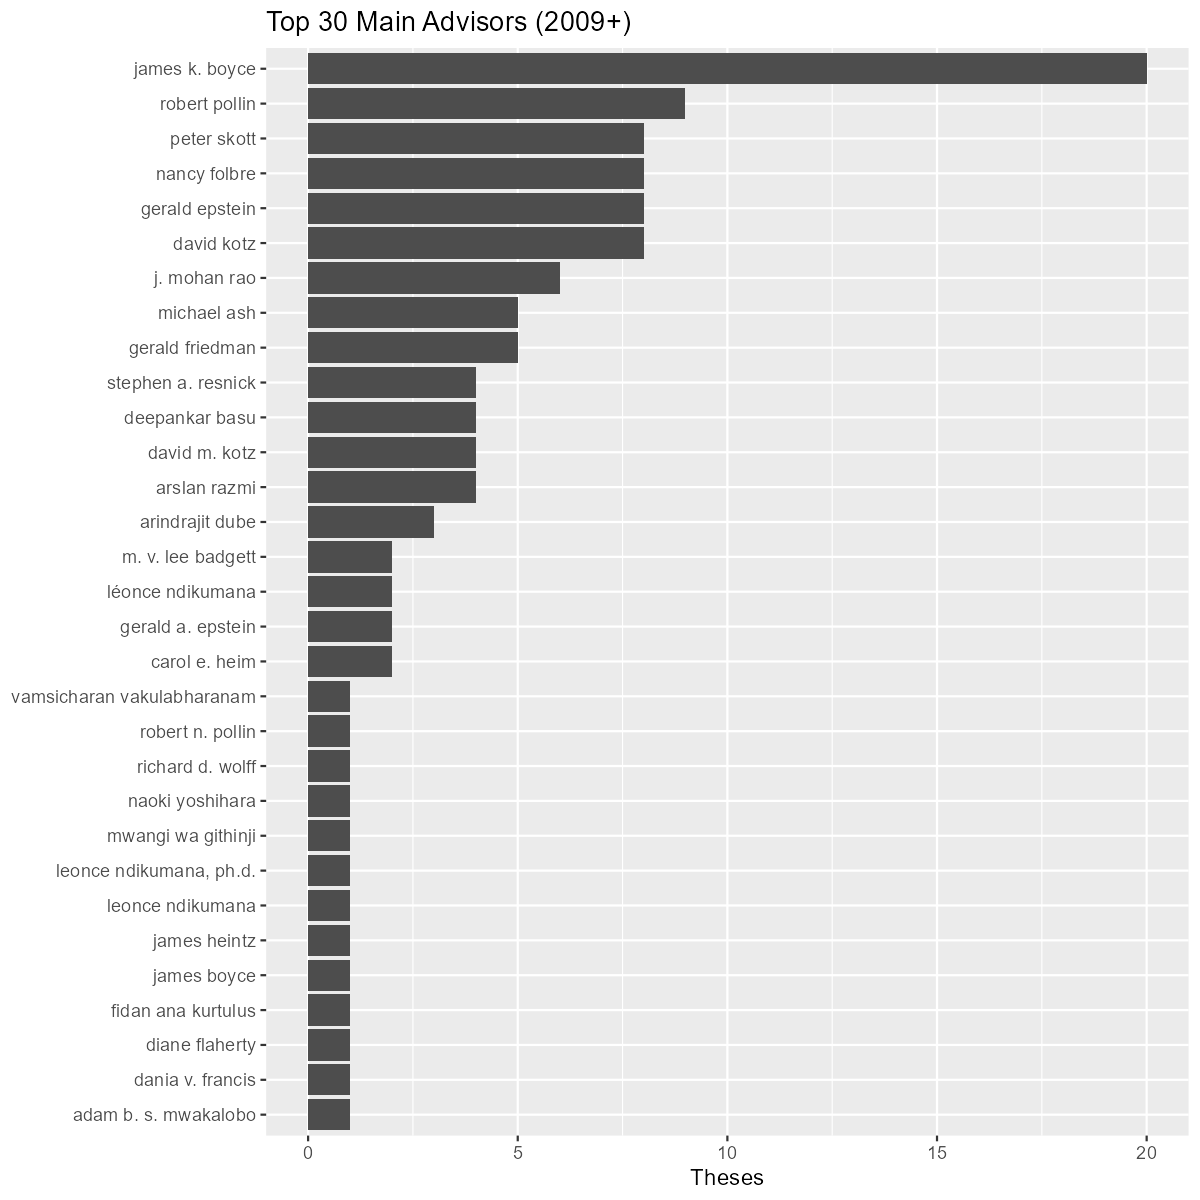
\includegraphics[width=\linewidth]{top_main_advisors.png}
		\caption{Top 30 \textit{main advisors} (2009--presente).}
	\end{figure}
	
	\section{Zoom al corpus de abstracts de sus estudiantes}
	Para explorar el contenido temático, filtré todas las tesis en las que Boyce aparece como advisor en cualquier rol (adv1..adv5). Se limpiaron los textos removiendo \textit{stopwords} en inglés y términos poco informativos (\textit{dissertation}, \textit{chapter}, \textit{also}, \textit{can}, siglas como \textit{cfm} y \textit{csa}). Luego se tokenizó en unigramas y bigramas y se combinaron las frecuencias para una lectura compacta.
	
	\section{Lectura de la nube de palabras}
	La nube resultante muestra un patrón claro:
	\begin{itemize}
		\item Eje ambiental--desarrollo: \textit{environmental}, \textit{development}, \textit{economic}, \textit{pollution}.
		\item Ingreso y distribución: \textit{income}, \textit{inequality}, \textit{poverty}.
		\item Territorio y hogares: \textit{rural}, \textit{households}, \textit{community}, \textit{local}, \textit{food}.
		\item Trabajo y género: \textit{employment}, \textit{labor}, \textit{women}.
		\item Enfoque empírico: \textit{data}, \textit{analysis}, \textit{study}, \textit{evidence}.
	\end{itemize}
	En suma, el corpus asociado a Boyce articula economía del medio ambiente, desarrollo y equidad, con anclaje empírico y atención a hogares, comunidades y mercados laborales.
	
	\begin{figure}[H]\centering
		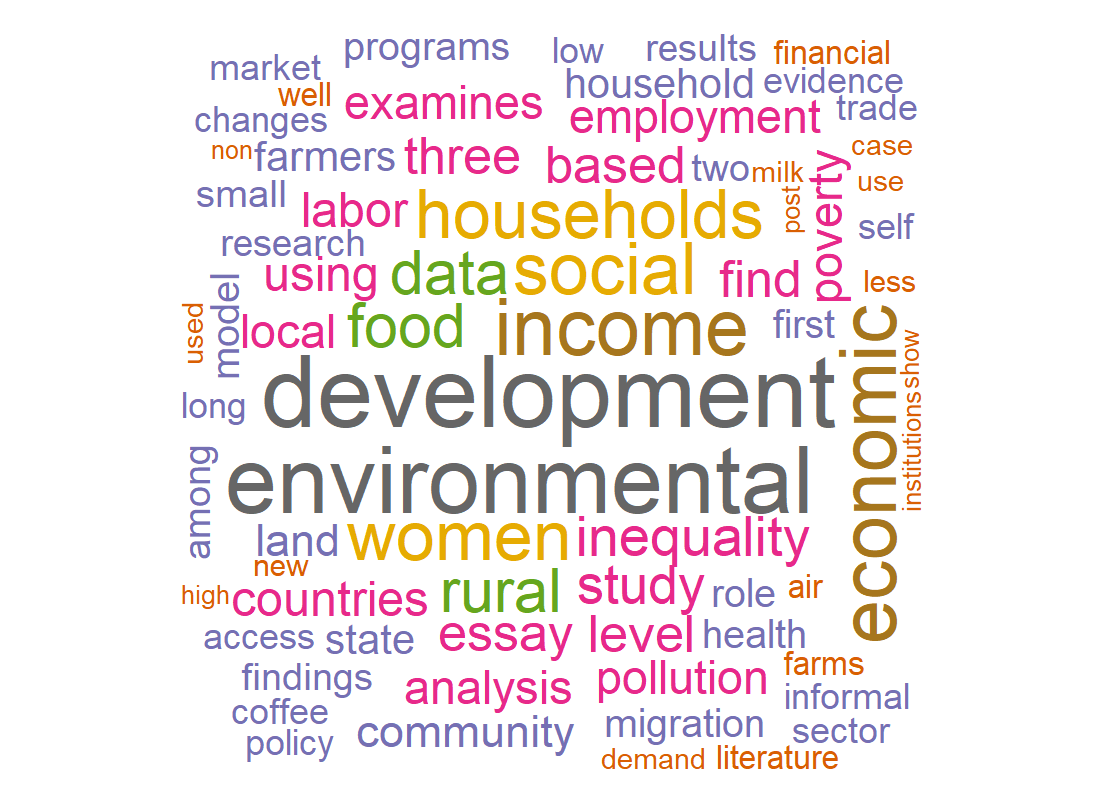
\includegraphics[width=\linewidth]{wordcloud_boyce_unigrams_bigrams.png}
		\caption{Nube de palabras (unigramas + bigramas) de abstracts de tesis con James K.~Boyce como advisor.}
	\end{figure}
	
	\section*{Notas técnicas mínimas}
	Las figuras se generaron en \texttt{R} con \texttt{tidyverse}, \texttt{tidytext}, \texttt{stopwords}, \texttt{wordcloud}. El ranking usa adv1; la nube agrega unigramas y bigramas tras limpieza de stopwords y términos irrelevantes.
	
\end{document}
